\documentclass[12pt,a4paper]{article}
\synctex=1
\usepackage[utf8]{inputenc}
\usepackage[margin=1cm]{geometry}
\usepackage{graphicx}
%\usepackage{verbatim}
\usepackage{amsmath}
\usepackage{amsfonts}
\usepackage{amssymb}
\usepackage{listings}
\usepackage{enumitem}
\usepackage{textcomp}
\usepackage{courier}
\usepackage{libertine}
\usepackage{pgfornament}
\usepackage{eso-pic}
\usepackage[hangul]{kotex}
\linespread{1.3}

\title{
	\centering
	\pgfornament[width=12cm,color=teal]{84}\\
	\vspace{1cm}
	\fontsize{50}{50} \selectfont {정보통신 수학 및 실습\\Lab assignment}\\
		\pgfornament[width=12cm,color=teal]{88}\\
	\vfill}
\author{
	\LARGE
	\begin{tabular}{rcc}
		\hline
		학번 : & 2016110056 & 2012112130\\ 
		이름 : & 박승원 & 노희승\\
		편성 : & 20조 & \today\\
		\hline
	\end{tabular}\vspace{1cm}
	\\

\includegraphics[width=0.5\textwidth]{logo.jpg}
	}
\date{}

\begin{document}
\maketitle
\pagenumbering{gobble}
\noindent
\lstset{language=matlab, columns=flexible, tabsize=4, frame=shadowbox, showstringspaces=false, breaklines=true, upquote=true, basicstyle=\normalsize}

\renewcommand{\thesubsubsection}{\alph{subsubsection})}
\renewcommand{\thesubsection}{\arabic{subsection}.}
\newpage
\section*{Chapter 8 Lab Assignment}

\subsection{If the outlet is a pipe that discharges to atmospheric pressure pa and provides a resistance, R, to flow that is proportional to the pressure difference across its ends, then find the outlet flow rate qmo and the differential equation of h(t).  Hint: qmo is (1/R)* (the pressure difference across its ends).\\Now solve your differential equation of h(t) using MATLAB and plot h(t) against the time.  The values of the parameters are as follows: (units are ignored)\\qmi = 25, R = 5, A = 10, h(0) = 10, ρ = 2.}
\begin{gather*}
q_{mo} = q_{mi} - \rho A \frac{dh}{dt}=\frac{1}{R}P = \frac{\rho h(t)}{R}\\
q_{mi}-\rho A \frac{dh(t)}{dt} = \frac{\rho h(t)}{R}\\
\frac{1}{A}(\frac{q_{mi}}{\rho} - \frac{h(t)}{R}) =  \frac{dh(t)}{dt}\\
\frac{1}{A}(\frac{q_{mi}}{\rho} - \frac{h(t)}{R}) = \frac{h(t+\Delta t)-h(t)}{\Delta t} \\
h(t + \Delta t) = \frac{\Delta t}{A}(\frac{q_{mi}}{\rho} - \frac{h(t)}{R}) + h(t)\\
h(k+1) = \frac{\Delta t}{A}(\frac{q_{mi}}{\rho} - \frac{h(k)}{R}) + h(k)\\
\end{gather*}
\lstinputlisting{1.m}
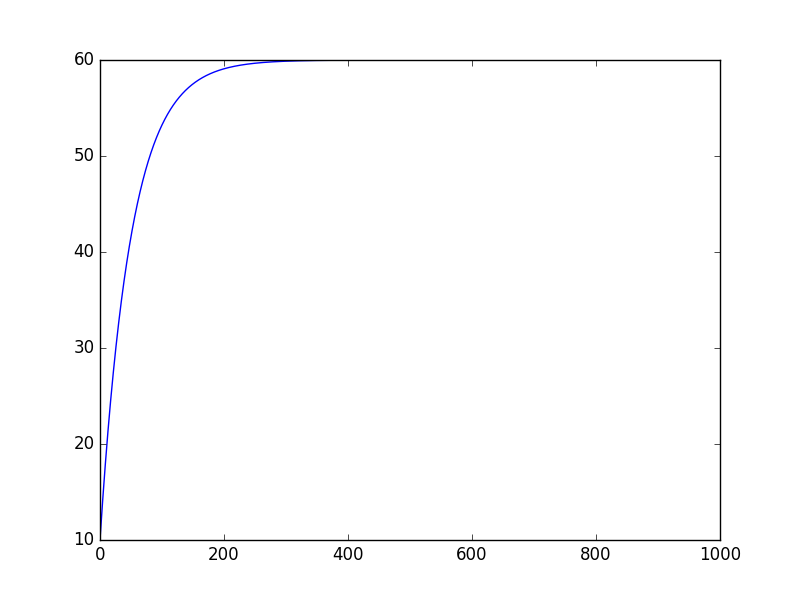
\includegraphics[width=0.8\textwidth]{11.png}
	
\subsection{Solve the following 2 order differential equation using MATLAB.\\$	y'' +2y' +y = 0, y(0) = 1, y'(0) = 3$}
\begin{gather*}
y''(t) + 2y'(t) + y(t) = 0\\
y'(t) = z(t)\\
\frac{y(t+\Delta t) - y(t)}{\Delta t} = z(t)\\
y(k+1) = z(k)\Delta t + y(k)\\
z'(t) + 2z(t) + y(t) = 0\\
\frac{z(t+\Delta t) - z(t)}{\Delta t} + 2z(t) + y(t) = 0\\
z(k+1) = -\Delta t(2z(k) + y(k)) + z(k)\\ 
z(0) = 3\\
\end{gather*}
\lstinputlisting{2.m}
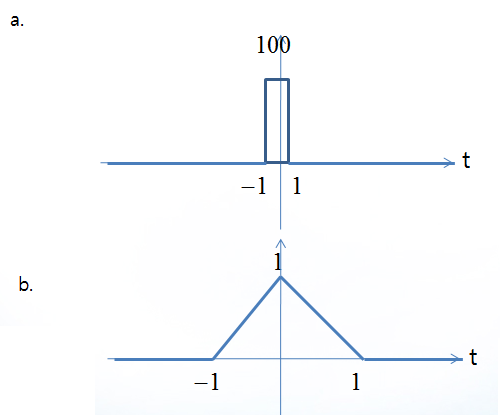
\includegraphics[width=0.7\textwidth]{1.png}
\subsection{For the following differential equation, solve the response y[n] when x[n] is the sampling values of sin(2*pi*t),  0≤t≤2*pi,  Δt=0.01.  Plot y[n] and x[n] against n.\\y[n] = 0.7*x[n] + 0.3*x[n-1]} 
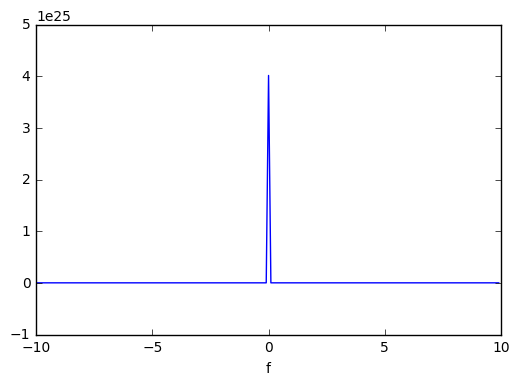
\includegraphics[width=0.8\textwidth]{4.png}
\end{document}
